\section{Expériences de Young}}

FIXME ajouter biographie de Thomas Young

\subsection{Mise en évidence du comportement ondulatoire de la
lumière.}

\subsubsection{Interférences d'un son (onde sonore)}

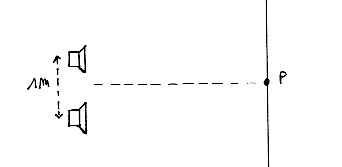
\includegraphics[width=7.922cm,height=3.875cm]{Pictures/1000000100000156000000A71108C5553D5F186E.png}

\paragraph{Exemple 1}

Deux haut-parleurs sont distants de 1 mètre et émettent chacun un son
d'une fréquence égale à 1000 Hz en concordance de phase.

Comment sera l'intensité du son perçu au point P ?

\begin{figure}
\centering
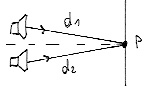
\includegraphics[width=4.12cm,height=2.434cm]{Pictures/100000010000009E0000005DF543EBD570977663.png}
\caption{}
\end{figure}

Réponse~:
P est situé en un point tel que $S_1$= 
la différence de marche $d_{2} - d_{1}$ est
nulle et donc les ondes arrivent au point P en concordance de phase. Il
s'agit d'un point d'interférence constructive et l'intensité du son en P
sera maximale.

\begin{figure}
\centering
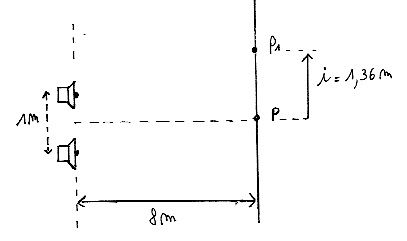
\includegraphics[width=7.154cm,height=4.233cm]{Pictures/1000000100000197000000F1DA056A96FDEF75DB.png}
\caption{}
\end{figure}

\paragraph{Exemple 2}

Deux haut-parleurs sont distants de 1 mètre et émettent chacun un son
d'une fréquence égale à 1000 Hz en concordance de phase.

Comment sera l'intensité du son perçu au point P1 si ce point se trouve
à une distance i=1,36 m du point P?

\begin{figure}
\centering
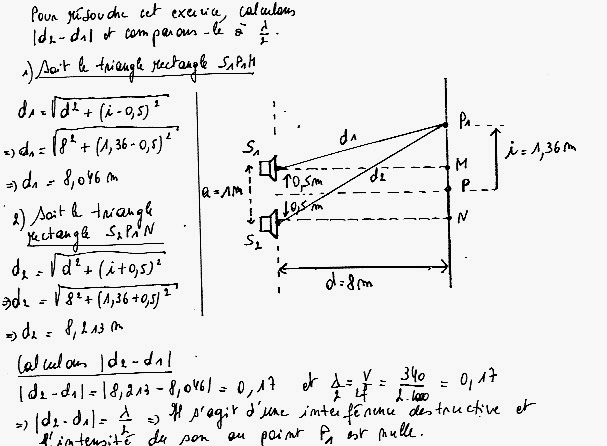
\includegraphics[width=15.545cm,height=11.171cm]{Pictures/100000010000025F000001BE110A2F11D2815100.png}
\caption{}
\end{figure}

\subsubsection{Généralisation}

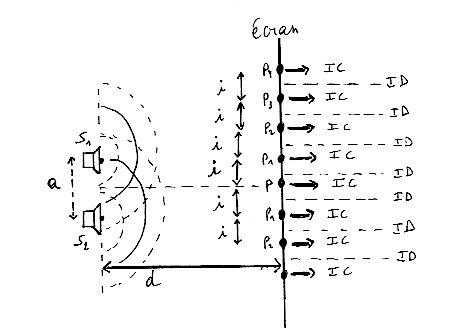
\includegraphics[width=7.086cm,height=5.068cm]{Pictures/10000001000001CB00000148F2D7DB2B0F2EC580.png}

Nous
voyons donc que lorsque nous nous déplaçons sur la droite verticale (que
nous appellerons l'écran), nous parcourons une succession de zones
d'interférences constructives (IC) et d'interférences destructives (ID).

Les zones d'interférences constructives sont telles que l'intensité du
son est maximale et les zones d'interférences destructives, telles que
l'intensité du son est nulle. Elles sont séparées d'une distance i
(appelée interfrange)

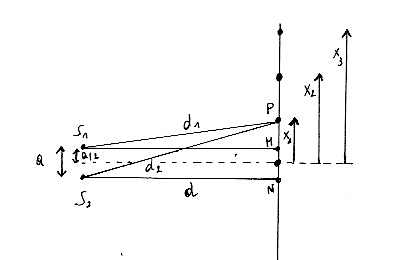
\includegraphics[width=8.123cm,height=5.352cm]{Pictures/100000010000018B00000104CBB3B40EFC3646D7.png}

La question est~: pouvons-nous trouver la distance qui sépare les zones
d'interférence constructives (l'interfrange $i$), en fonction de
$\delta$, a et d où~: 

\begin{description}
 \item{\delta}~: longueur d'onde des sons émis.
 \item{i}~: distance entre deux zones d'interférences constructives.
 \item{d}~: distance entre les sources et l'écran.
 \item{a}~: distance entre les deux sources.
\end{description}

Remarquez sur le schéma ci-contre~: $x_{1}=i$,
$x_{2}-x_{1} = i$,
$x_{3}-x_{2} = i$, \ldots.

$x$ est la distance entre le point central et un point d'interférence
constructive.

\begin{figure}
\centering
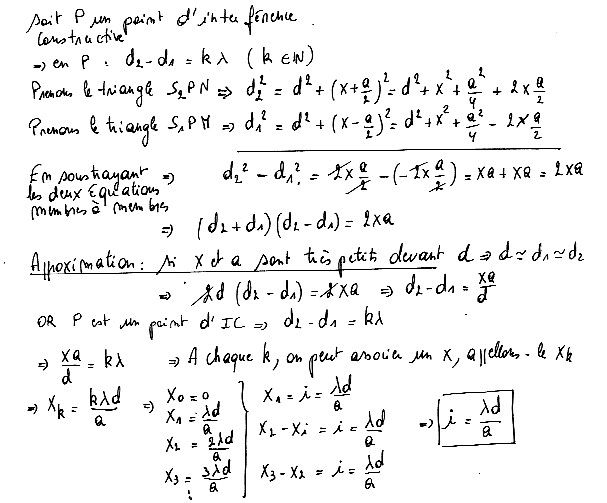
\includegraphics[width=17.253cm,height=13.09cm]{Pictures/100000010000025F000001F704069EFE234008BD.png}
\caption{}
\end{figure}

\subsubsection{Interférence lumineuse }

\paragraph{Expérience de Young~: diffraction à travers deux fentes
et figure d'interférences. }

Nous venons de voir que les interférences sonores sont caractéristiques
d'un comportement ondulatoire.

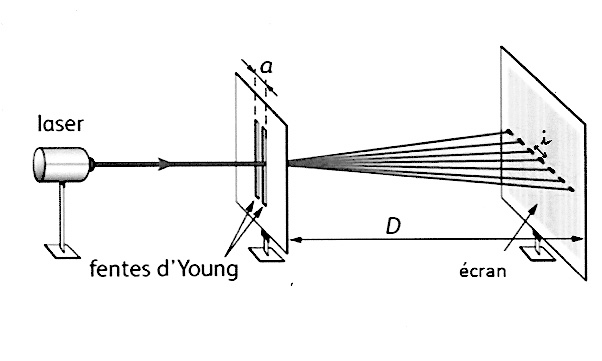
\includegraphics[width=10.592cm,height=6.443cm]{Pictures/100000010000025A000001696E99605075C8F3D0.png}

\emph{Que se passera-t-il si nous soumettons la lumière à cette expérience
d'interférence~? }

Décrivons cette expérience, \emph{l'expérience de Young.}

De la lumière provenant d'un laser traverse un écran percé de deux
fentes fines, distantes d'une courte distance a (les fentes de Young).

Sur un écran, situé à une distance D des fentes, on observe une
succession de points lumineux, séparés par une distance i.

\begin{figure}
\centering
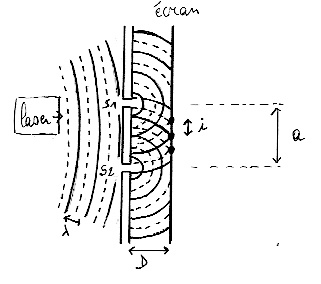
\includegraphics[width=8.299cm,height=7.35cm]{Pictures/10000001000001410000011C9E9E805F9A9605B7.png}
\caption{}
\end{figure}

\emph{Interprétation }

En analogie avec deux sources d'ondes sonores, nous pouvons conclure que
seul le modèle ondulatoire peut expliquer ces observations.

Les deux fentes de Young S1 et S2 vont se comporter comme de nouvelles
sources et diffracter la lumière incidente provenant du laser.

Ces deux ondes vont produire des interférences sur l'écran et produire
une succession de points lumineux.

Les points lumineux sont des zones d'interférences constructives et
entre les points lumineux, l'absence de lumière, correspond à des zones
d'interférences destructives, ce qui est typiquement un comportement
ondulatoire.

Nous avons démontré précédemment, dans le cas d'interférences de deux
ondes sonores, le lien qui relie , i, a et D. En suivant une démarche
identique pour cette expérience de Young, nous obtenons la relation~:

\begin{figure}
\centering
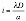
\includegraphics[width=1.788cm,height=1.46cm]{Pictures/100000010000001A00000015860A63C6525557ED.png}
\caption{}
\end{figure}

Dans notre situation~: i et a sont très petits devant D, l'approximation
est très pertinente (voir démonstration).

L'expérience de Young avec de la lumière conduit à la même relation~:

\emph{\textbf{Cette expérience montre que la lumière a un caractère
ondulatoire et donc que la lumière}}

\emph{\textbf{se comporte comme une onde. Elle est donc caractérisée par
une fréquence f et une longueur d'onde }\textbf{}\textbf{.}}

\emph{\textbf{b) }\textbf{Calcul angulaire de la position des points
d'interférence constructive}}

\begin{figure}
\centering
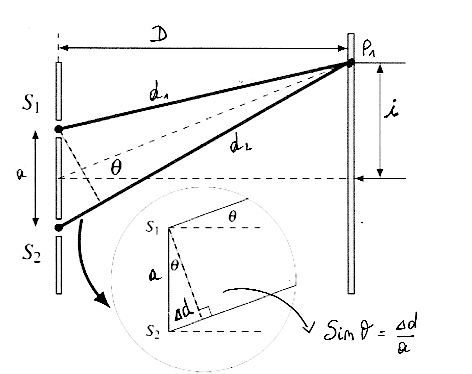
\includegraphics[width=7.071cm,height=5.604cm]{Pictures/10000001000001D8000001766572F750E44C7125.png}
\caption{}
\end{figure}

Soit P\textsubscript{1}, un point d'interférence constructive situé
juste après le point central, notons θ la position angulaire de ce
point.

En ce point P\textsubscript{1}, l'interférence étant constructive, la
différence de marche d= d\textsubscript{2} -- $S_1$ =


En faisant l'approximation déjà réalisée précédemment, à savoir~: a et i
 D, nous pouvons considérer que les rayons lumineux d1 et d2 sont
quasiment parallèles.

En considérant le triangle rectangle représenté sur le schéma~:

d= = a Sin θ

\begin{figure}
\centering
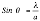
\includegraphics[width=2.095cm,height=1.107cm]{Pictures/100000010000002800000015DDF3AE193165C3E3.png}
\caption{}
\end{figure}

Nous avons donc que~:  = a Sin θ et donc~:

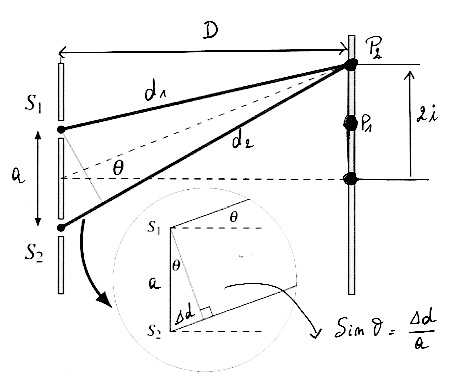
\includegraphics[width=5.061cm,height=4.096cm]{Pictures/10000001000001D80000017E98931F1CF545D918.png}\emph{\textbf{Généralisation
}}

- Considérons un point P\textsubscript{2}

En ce point P\textsubscript{2 }, l'interférence étant constructive, la
différence de marche d= d\textsubscript{2} -- $S_1$ =
2

En considérant le triangle rectangle représenté sur le schéma~: d= =
a Sin θ

Donc~:
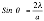
\includegraphics[width=2.306cm,height=1.107cm]{Pictures/100000010000002C000000153ADDDC592928E9B8.png}

En continuant le raisonnement de la sorte pour des points~:

P\textsubscript{3} distant de 3i du point central,

P\textsubscript{4} distant de 4i du point central,

P\textsubscript{5} distant de 5i du point central, \ldots{}

\begin{figure}
\centering
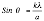
\includegraphics[width=2.306cm,height=1.107cm]{Pictures/100000010000002C0000001558E0CCA95D4F59EB.png}
\caption{}
\end{figure}

Nous arrivons à~:

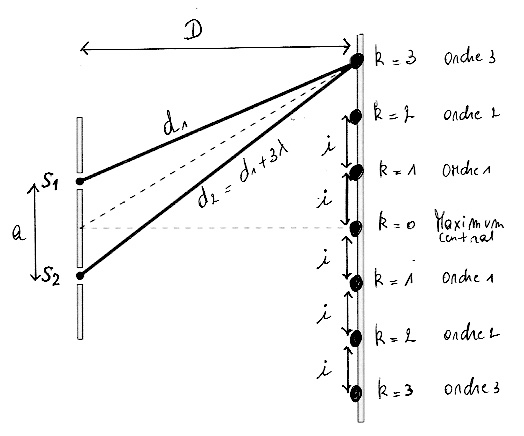
\includegraphics[width=7.086cm,height=5.897cm]{Pictures/100000010000020C000001B4676C159EC881E6E3.png}\emph{\textbf{Synthèse:}}

\begin{figure}
\centering
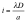
\includegraphics[width=1.757cm,height=1.432cm]{Pictures/100000010000001A000000159D382765312EA964.png}
\caption{}
\end{figure}

\begin{figure}
\centering
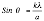
\includegraphics[width=2.894cm,height=1.389cm]{Pictures/100000010000002C0000001558E0CCA95D4F59EB.png}
\caption{}
\end{figure}

\emph{\textbf{4)Applications}}

\emph{\textbf{3.1 Détermination expérimentale de la longueur d'onde de
la lumière. }}

L'expérience de Young permet de déterminer la fréquence de la lumière

a) Réalisons l'expérience de Young avec une lumière jaune et les données
suivantes~:

D=1,75 m

a=1 mm

i~=1 mm

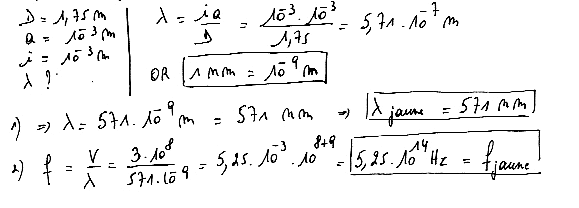
\includegraphics[width=16.82cm,height=5.733cm]{Pictures/1000000100000243000000D01464CBCF0F7AAEC1.png}Calculez
la longueur d'onde de la lumière jaune ainsi que la fréquence de la
lumière correspondante.

b)\textbf{ }Réalisons l'expérience de Young avec une lumière verte
sachant que l'expérience de Young nous fournit les valeurs suivantes~:

D=4,95 m

a=0,2 mm

i~=1,32 cm

Calculez la longueur d'onde de la lumière verte ainsi que la fréquence
de la lumière correspondante. Exprimez votre réponse en nm.

\begin{figure}
\centering
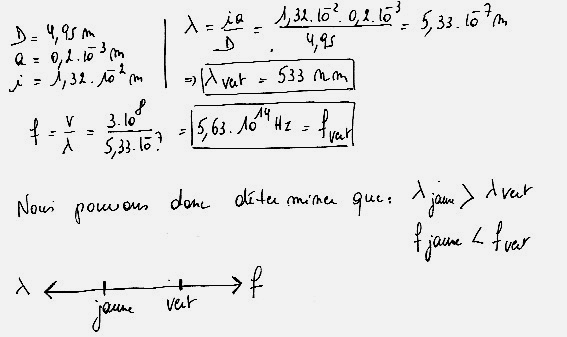
\includegraphics[width=15.833cm,height=8.654cm]{Pictures/100000010000023700000151168D50BCCC321003.png}
\caption{}
\end{figure}

\emph{\textbf{c) Le spectre de la lumière blanche}}

\emph{\textbf{Ces expériences nous montrent que chaque couleur de la
lumière possède une longueur d'onde et donc une fréquence
caractéristique de la couleur. }}

\textbf{}\textsubscript{\textbf{jaune}}\textbf{ 
}\textsubscript{\textbf{vert}}\textbf{ et donc
f}\textsubscript{\textbf{jaune}}\textbf{ 
f}\textsubscript{\textbf{vert}}

Or la lumière blanche est composée de toutes les couleurs de l'arc en
ciel. L'expérience de Young nous permet donc de classer toutes les
couleurs qui composent la lumière blanche en fonction de leur longueur
d'onde ( et donc de leur fréquence).

C'est ce qu'on appelle \emph{\textbf{le spectre de la lumière blanche.
(voir livre p 115)}}

\begin{figure}
\centering
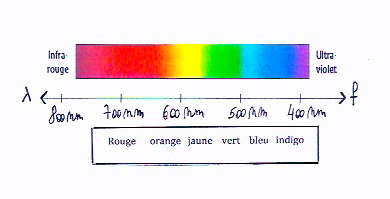
\includegraphics[width=11.557cm,height=5.907cm]{Pictures/1000000100000186000000C7B42157D8D8096212.png}
\caption{}
\end{figure}

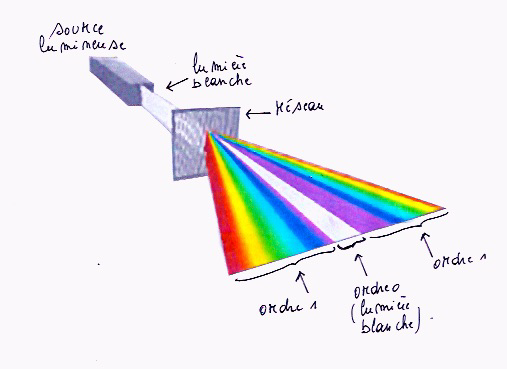
\includegraphics[width=9.176cm,height=6.676cm]{Pictures/10000001000001FB0000017167AEF9D1A02E0A78.png}\emph{\textbf{d)
Diffraction de la lumière blanche}}

Si on réalise l'expérience de diffraction de la lumière blanche par un
réseau, on observe que chaque couleur présentera ses maximums à un angle
différent, sauf pour le maximum central qui est à la même position (θ =
0) pour toutes les couleurs.

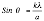
\includegraphics[width=2.259cm,height=1.082cm]{Pictures/100000010000002C0000001558E0CCA95D4F59EB.png}Les
plus grandes longueurs d'onde subiront les plus grandes déviations.

\textbf{Le maximum d'ordre 1 du mauve sera celui le plus près du
maximum} central puisque c'est la longueur d'onde visible la plus petite
alors que \textbf{le maximum d'ordre 1 le plus éloigné du maximum
central sera celui du rouge} puisque c'est cette couleur du visible qui
a la plus grande longueur d'onde. On aura alors la figure d'interférence
ci-contre.

\emph{\textbf{Applications~: }}

Les plumes si colorées de certains oiseaux.

\emph{\textbf{EXERCICES}}

\hypertarget{exercice-1}{%
\section{\texorpdfstring{\emph{Exercice
1}}{Exercice 1}}\label{exercice-1}}

De la lumière de longueur d'onde égale à 600 nm éclaire, suivant la
normale, deux fentes séparées de 0,1 mm.

\begin{enumerate}
\def\labelenumi{\alph{enumi})}
\tightlist
\item
  Quelle est la position angulaire d'ordre 1? (Rép~: 0,34°)
\item
  A quelle distance du point central se trouve ce maximum d'ordre 1~sur
  un écran situé à 3 mètres des fentes? (Rép~: 18 mm)
\end{enumerate}

\begin{quote}
\emph{\textbf{Exercice 2}}
\end{quote}

\begin{quote}
\end{quote}

\begin{quote}
On fait passer de la lumière ayant une longueur d'onde de 500 nm à
travers deux fentes séparées de 0,01 mm. On observe la figure de
diffraction sur un écran situé à 2 m de la fente.
\end{quote}

\begin{quote}
a) Quelle est la distance entre le maximum central et le premier
minimum? (Rép~: 5 cm)
\end{quote}

\begin{quote}
b) Quelle est la distance entre le maximum central et le deuxième
minimum? (Rép~: 15 cm)
\end{quote}

\begin{quote}
\end{quote}

\begin{quote}
\emph{\textbf{Exercice 3}}
\end{quote}

\begin{quote}
On fait passer des micro-ondes à travers deux fentes séparées de 1 cm.
Sur un écran situé à 1,6 m de distance de la fente, on observe une
interfrange de 50 cm. Quelle est la longueur d'onde des micro-ondes?
(Rép~: 3 mm)
\end{quote}

\begin{quote}
\end{quote}

\begin{quote}
\emph{\textbf{Exercice 4}}
\end{quote}

\begin{quote}
Dans une expérience de Young, la longueur d'onde de la lumière est de
500 nm. La distance entre les fentes est de 0,1 mm et on observe la
figure d'interférence sur un écran situé à 1,6 m des fentes. Quel est
l'angle entre le maximum central et le maximum d'ordre 5? (Rép~: 1,43°)
\end{quote}

\begin{quote}
\end{quote}

\begin{quote}
\emph{\textbf{Exercice 5}}
\end{quote}

\begin{quote}
Dans une expérience de Young, la longueur d'onde de la lumière est de
600 nm.
\end{quote}

\begin{quote}
On remarque alors que le maximum d'ordre 4 est à 1 cm du maximum central
sur un écran situé à 2 m des fentes. Quelle est la distance entre les
fentes\textbf{ }? (Rép~: 0,48 mm)
\end{quote}

\begin{quote}
\end{quote}

\begin{quote}
\emph{\textbf{Exercice 6}}
\end{quote}

\begin{quote}
Au cours d' une expérience de Young, la longueur d'onde de la lumière
est de 632 nm et
\end{quote}

\begin{quote}
la distance entre les fentes est de 0,2 mm. La figure montre la figure
d'interférence
\end{quote}

\begin{quote}
qu'on observe sur un écran. À quelle distance des fentes est situé
l'écran\textbf{ }? (Rép~: 1,46 m)
\end{quote}

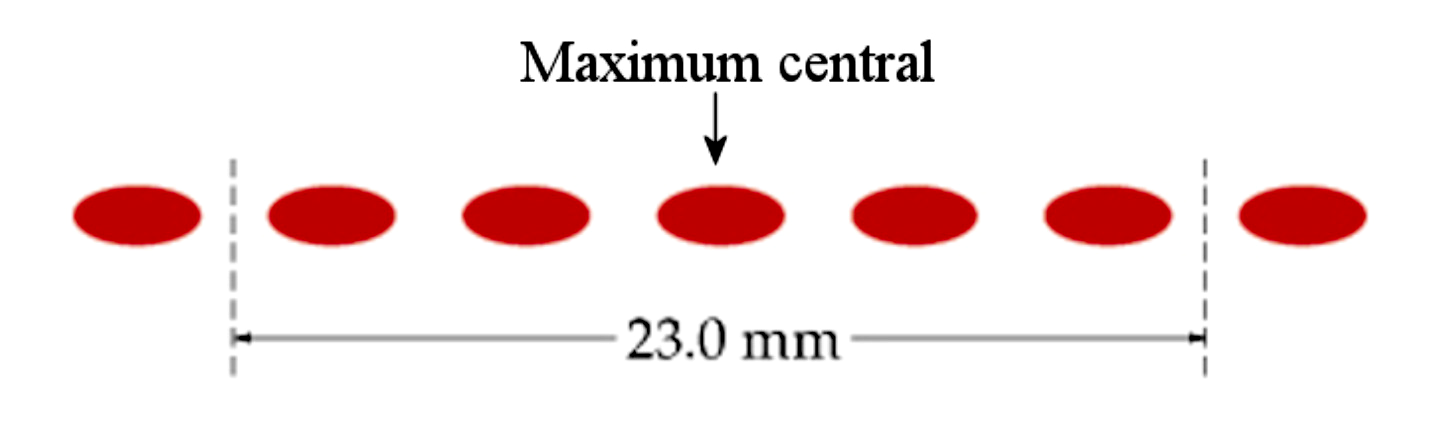
\includegraphics[width=13.259cm,height=4.045cm]{Pictures/100000010000059F000001B75001F99348A6D888.png}

\emph{\textbf{EXERCICES}}

\hypertarget{exercice-1-1}{%
\section{\texorpdfstring{\emph{Exercice
1}}{Exercice 1}}\label{exercice-1-1}}

De la lumière de longueur d'onde égale à 600 nm éclaire, suivant la
normale, deux fentes séparées de 0,1 mm.

a) Quelle est la position angulaire du maximum d'ordre 1~?

b) A quelle distance du point central se trouve ce maximum d'ordre 1~sur
un écran situé à 3 mètres des fentes?

\begin{quote}
\emph{\textbf{Exercice 2}}
\end{quote}

\begin{quote}
\end{quote}

\begin{quote}
On fait passer de la lumière ayant une longueur d'onde de 500 nm à
travers deux fentes séparées de 0,01 mm. On observe la figure de
diffraction sur un écran situé à 2 m de la fente.
\end{quote}

\begin{quote}
\end{quote}

\begin{quote}
a) Quelle est la distance entre le maximum central et le premier
minimum?
\end{quote}

\begin{quote}
\end{quote}

\begin{quote}
\end{quote}

\begin{quote}
\end{quote}

\begin{quote}
\end{quote}

\begin{quote}
\end{quote}

\begin{quote}
b) Quelle est la distance entre le maximum central et le deuxième
minimum?
\end{quote}

\begin{quote}
\end{quote}

\begin{quote}
\end{quote}

\begin{quote}
\end{quote}

\begin{quote}
\end{quote}

\begin{quote}
\end{quote}

\begin{quote}
\end{quote}

\begin{quote}
\end{quote}

\begin{quote}
\emph{\textbf{Exercice 3}}
\end{quote}

\begin{quote}
On fait passer des micro-ondes à travers deux fentes séparées de 1 cm.
Sur un écran situé à 1,6 m de distance de la fente, on observe une
interfrange de 50 cm. Quelle est la longueur d'onde des micro-ondes?
\end{quote}

\begin{quote}
\end{quote}

\begin{quote}
\end{quote}

\begin{quote}
\end{quote}

\begin{quote}
\end{quote}

\begin{quote}
\end{quote}

\begin{quote}
\end{quote}

\begin{quote}
\end{quote}

\begin{quote}
\end{quote}

\begin{quote}
\end{quote}

\begin{quote}
\end{quote}

\begin{quote}
\end{quote}

\begin{quote}
\emph{\textbf{Exercice 4}}
\end{quote}

\begin{quote}
Dans une expérience de Young, la longueur d'onde de la lumière est de
500 nm. La distance entre les fentes est de 0,1 mm et on observe la
figure d'interférence sur un écran situé à 1,6 m des fentes. Quel est
l'angle entre le maximum central et le maximum d'ordre 5? (Rép~:
\end{quote}

\begin{quote}
\end{quote}

\begin{quote}
\end{quote}

\begin{quote}
\end{quote}

\begin{quote}
\end{quote}

\begin{quote}
\end{quote}

\begin{quote}
\end{quote}

\begin{quote}
\end{quote}

\begin{quote}
\end{quote}

\begin{quote}
\end{quote}

\begin{quote}
\end{quote}

\begin{quote}
\end{quote}

\begin{quote}
\emph{\textbf{Exercice 5}}
\end{quote}

\begin{quote}
Dans une expérience de Young, la longueur d'onde de la lumière est de
600 nm.
\end{quote}

\begin{quote}
On remarque alors que le maximum d'ordre 4 est à 1 cm du maximum central
sur un écran situé à 2 m des fentes. Quelle est la distance entre les
fentes\textbf{ }? (Rép~:
\end{quote}

\begin{quote}
\end{quote}

\begin{quote}
\end{quote}

\begin{quote}
\end{quote}

\begin{quote}
\end{quote}

\begin{quote}
\end{quote}

\begin{quote}
\end{quote}

\begin{quote}
\end{quote}

\begin{quote}
\end{quote}

\begin{quote}
\end{quote}

\begin{quote}
\end{quote}

\begin{quote}
\end{quote}

\begin{quote}
\end{quote}

\begin{quote}
\emph{\textbf{Exercice 6}}
\end{quote}

\begin{quote}
Au cours d' une expérience de Young, la longueur d'onde de la lumière
est de 632 nm et
\end{quote}

\begin{quote}
la distance entre les fentes est de 0,2 mm. La figure montre la figure
d'interférence
\end{quote}

\begin{quote}
qu'on observe sur un écran. À quelle distance des fentes est situé
l'écran\textbf{ }? (Rép~:
\end{quote}

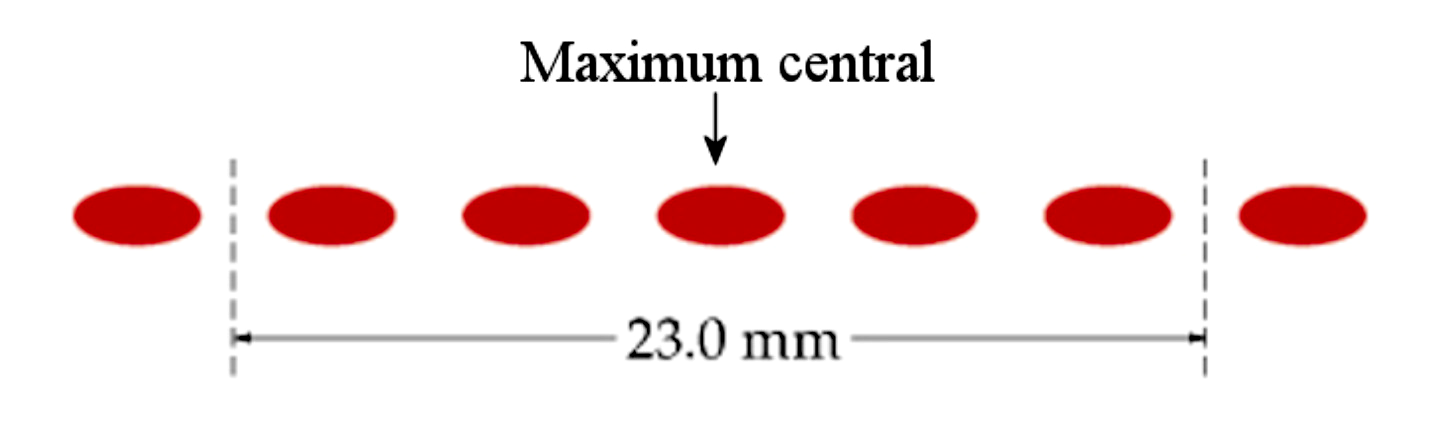
\includegraphics[width=13.259cm,height=4.045cm]{Pictures/100000010000059F000001B75001F99348A6D888.png}

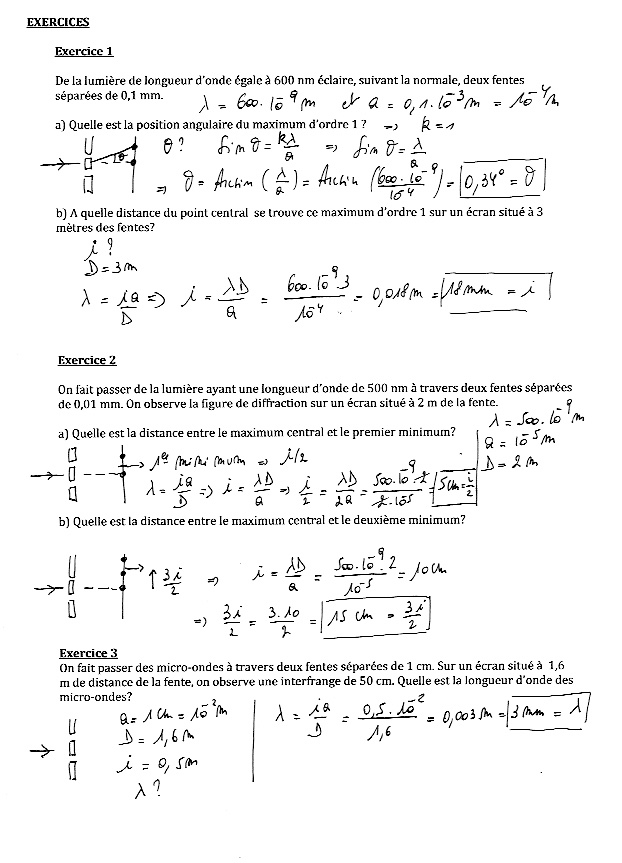
\includegraphics[width=18.503cm,height=25.663cm]{Pictures/100000010000026E0000035F0050AD553CE14CB4.png}

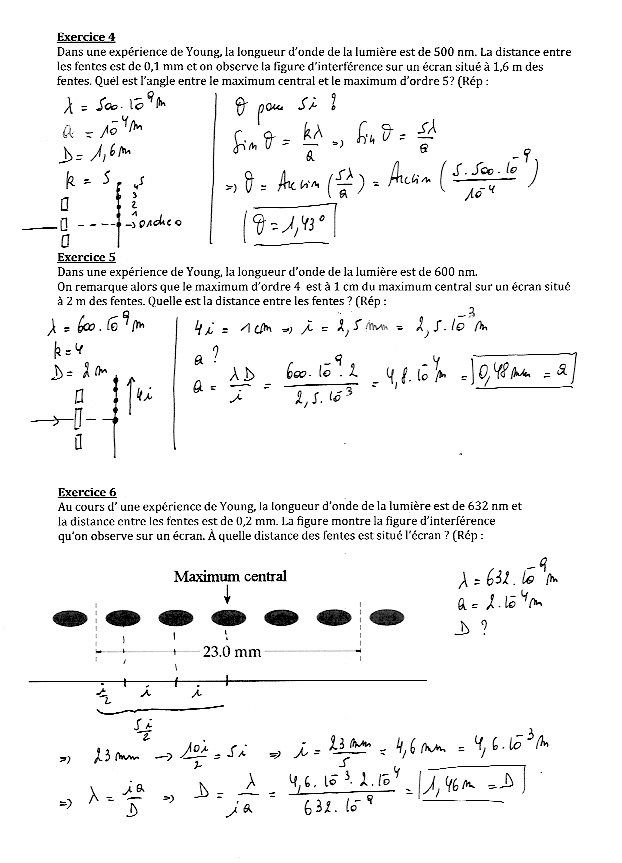
\includegraphics[width=18.503cm,height=25.663cm]{Pictures/100000010000026E0000035F170A4BD46BAD55A6.png}
